\documentclass[12pt,a4paper,oneside]{article}

\usepackage[utf8]{inputenc}
\usepackage[portuguese]{babel}
\usepackage[T1]{fontenc}
\usepackage{amsmath}
\usepackage{amsfonts}
\usepackage{amssymb}
\usepackage{graphicx}

\usepackage{xcolor}
% Definindo novas cores
\definecolor{verde}{rgb}{0.25,0.5,0.35}
\definecolor{jpurple}{rgb}{0.5,0,0.35}
% Configurando layout para mostrar codigos Java
\usepackage{listings}
\lstset{
  language=Java,
  basicstyle=\ttfamily\small, 
  keywordstyle=\color{jpurple}\bfseries,
  stringstyle=\color{red},
  commentstyle=\color{verde},
  morecomment=[s][\color{blue}]{/**}{*/},
  extendedchars=true, 
  showspaces=false, 
  showstringspaces=false, 
  numbers=left,
  numberstyle=\tiny,
  breaklines=true, 
  backgroundcolor=\color{cyan!10}, 
  breakautoindent=true, 
  captionpos=b,
  xleftmargin=0pt,
  tabsize=4,
  escapeinside=||
}

\author{\\Universidade Federal de Jataí (UFJ)\\Bacharelado em Ciência da Computação \\Inteligência Artificial \\Esdras Lins Bispo Jr.}

\title{\sc \huge Segunda Prova}

\begin{document}

\maketitle

{\bf ORIENTAÇÕES PARA A RESOLUÇÃO}

\begin{itemize}
	\item A avaliação é individual, sem consulta;
	\item A pontuação máxima desta avaliação é 10,0 (dez) pontos, sendo uma das 04 (quatro) componentes que formarão a média final da disciplina: duas provas, um projeto e exercícios;
	\item A média final será calculada pela média ponderada das quatro supraditas notas [em que a primeira prova tem peso 40 (quarenta), a segunda prova tem peso 30 (trinta), o projeto tem peso 30 (trinta) e os exercícios-bônus são adicionados à media final];
	\item O somatório da pontuação de todas as questões desta avaliação é 11,0 (onze) pontos. Isto é um sinônimo de tolerância na correção. Se você por acaso perder 1,5 (um e meio), sua nota será 9,5 (nove e meio);
	\item O conteúdo exigido compreende os seguintes pontos apresentados no Plano de Ensino da disciplina: (1) Introdução à Inteligência Artificial, (2) Agentes Inteligentes, (3) Resolução de Problemas por meio de Busca, (4) Representação do Conhecimento, (5) Redes Neurais Artificiais, (6) Computação Natural, (7) Aprendizagem a partir de exemplos, (8) Mine\-ração de Dados, e (9) Outros Tópicos.
\end{itemize}

\begin{center}
	\fbox{\large Nome: \hspace{10cm}}
	\fbox{\large Assinatura: \hspace{9cm}}
\end{center}

\newpage

\begin{enumerate}


	\item[] \colorbox{black}{
		\color{white}Todas as questões necessitam não apenas
	}\\ 
	\colorbox{black}{
		\color{white} serem respondidas, mas também justificadas.
	}
		\item (3,0 pt) [ENADE 2008] Considere um jogo do tipo 8-$puzzle$, cujo objetivo é conduzir o tabuleiro esquematizado na figura abaixo para o seguinte estado final. 
		
		\begin{center}
			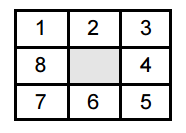
\includegraphics[width=4cm]{images/enade01}
		\end{center}
		
		Considere, ainda, que, em determinado instante do jogo, se tenha o estado $E0$ a seguir.
		
		\begin{center}
			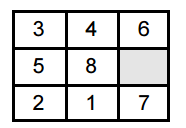
\includegraphics[width=4cm]{images/enade02}
		\end{center}
		
		Pelas regras desse jogo, sabe-se que os próximos estados possíveis são os estados $E1$, $E2$ e $E3$ mostrados abaixo.
		
		\begin{center}
			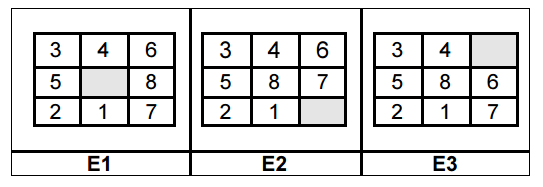
\includegraphics[width=10cm]{images/enade03}
		\end{center}
		
		Considere uma função heurística $h$ embasada na soma das distâncias das peças em relação ao estado final desejado,
		em que a distância $d$ a que uma peça $p$ está da posição final é dada pela soma do número de linhas com o número de colunas que a separam da posição final desejada. Por exemplo, em E1, $d(1) = 2 + 1 = 3$. A partir dessas informações analise as asserções a seguir.
		
		Utilizando-se um algoritmo de busca gulosa pela melhor escolha que utiliza a função h, o próximo estado no desenvolvimento do jogo a partir do estado $E0$ tem de ser $E3$.
		
		\begin{center}
			PORQUE
		\end{center}
		
		dos três estados $E1$, $E2$ e $E3$ possíveis, o estado com menor soma das distâncias entre a posição atual das peças e a posição final é o estado $E3$.
		
		\begin{enumerate}
			\item As duas asserções são proposições verdadeiras, e a segunda é uma justificativa correta da primeira.
			\item As duas asserções são proposições verdadeiras, e a segunda não é uma justificativa correta da primeira.
			\item A primeira asserção é uma proposição verdadeira, e a segunda é uma proposição falsa.
			\item A primeira asserção é uma proposição falsa, e a segunda é uma proposição verdadeira.
			\item As duas asserções são proposições falsas.
		\end{enumerate}
	
		\item (2,5 pt) Quatro pessoas precisam atravessar uma ponte que suporta no máximo duas pessoas ao mesmo tempo. É noite e eles não podem ver o caminho. Por sorte o grupo possui uma tocha que pode ser usada para iluminar o caminho enquanto eles atravessam a ponte. O tempo necessário para cada pessoa atravessar a ponte é respectivamente: 1, 2, 5 e 10 minutos. 
	
	\begin{enumerate}
		\item (1,5 pt) Descreva o problema em termos de um problema de busca definindo o espaço de estados, o estado inicial, estado final, os operadores de transição entre os estados (ações) e o custo.
		\item (1,0 pt) Quantas vezes, no mínimo, é necessário realizar a travessia da ponte?
	\end{enumerate}

\newpage

	\item (1,5 pt) {\bf [IpC Q016]} Sobre as redes neurais de múltiplas camadas, é \underline{incorreto} afirmar que...

\begin{enumerate}
\item a aprendizagem da rede é feita normalmente utilizando o algoritmo de propagação de retorno.
\item é possível existir uma ou várias camadas ocultas.
\item todos os neurônios das camadas ocultas recebem diretamente os valores de entrada.
\item ela é mais poderosa, em termos de classificação, do que as redes de única camada.
\end{enumerate}
	
	 \item (2,0 pt) {\bf [Vídeo sobre Agentes Lógicos]} Apresente um exemplo, dentro do mundo de Wumpus, exemplificando de que forma um agente inteligente pode utilizar a lógica no processo de tomada de decisão.
	 
	  \item (2,0 pt) {\bf [Vídeo sobre PLN]} Discorra sobre os níveis de análise textual. Detalhe especificamente dois deles, apresentando exemplos.
	
	
\end{enumerate}
\end{document}